\begin{figure}[H]
  \centering
  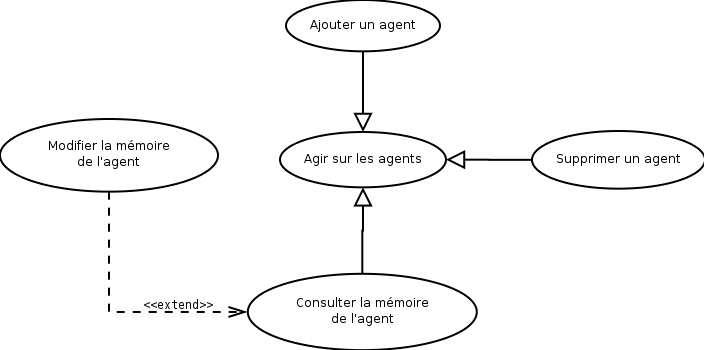
\includegraphics[width=14cm]{img/visidia_cu_agir_agent}
  \caption{Cas d'utilisation : Agir sur un agent} 
  \label{fig:cu_agir_agent}
\end{figure}

\subsubsection {Supprimer un agent pendant l'ex�cution}

\begin{tabular}{|l|p{10cm}|}
\hline
Cas d'utilisation 	& Supprimer un agent. \\
\hline
Acteur 			& L'utilisateur. \\
\hline 
But 			& Supprimer un agent du r�seau au moment de l'�xecution d'un algorithme. \\
\hline
R�sum� M�tier 		& L'utilisateur choisit un agent pour le supprimer.\\
\hline
Pr�-conditions 		& L'utilisateur dispose d'un agent dans le r�seau. \\
 \hline
Post-conditions 	& L'agent est supprim� du r�seau.\\
\hline
Commentaires 		& On ne peut supprimer qu'un seul agent � la fois.\\
\hline
\end{tabular}


\subsubsection {Ajouter un agent pendant l'ex�cution}

\begin{tabular}{|l|p{10cm}|}
\hline
Cas d'utilisation 	& Ajouter un agent. \\
\hline
Acteur 			& L'utilisateur. \\
\hline 
But           		& Ajouter un agent sur un sommet (non
�teint) dans un r�seau au moment de l'ex�cution d'un algorithme. \\
\hline

R�sum� M�tier 		& L'utilisateur choisit un sommet, il choisit
un agent parmi les agents qu'on a, puis il l'ajoute.\\ 
\hline
Pr�-conditions 		& L'utilisateur dispose d'un r�seau et d'une implantation d'agent. \\
 \hline
Post-conditions 	& L'agent est bien ajout� sur une sommet.\\
\hline
Commentaires 		& On ajoute un agent � l'unit�.\\
\hline
\end{tabular}

\subsubsection {Consulter un agent pendant l'ex�cution}

\begin{tabular}{|l|p{10cm}|}
\hline
Cas d'utilisation 	& consulter un agent. \\
\hline
Acteur 			& L'utilisateur. \\
\hline 
But 			& Consulter la m�moire d'un agent dans un r�seau au moment de l'ex�cution d'un algorithme. \\
\hline
R�sum� M�tier 		& L'utilisateur choisit un agent puis le consulte.\\
\hline
Pr�-conditions 		& L'utilisateur dispose d'un r�seau et d'une implantation d'agent. \\
 \hline
Post-conditions 	& L'agent est bien ajout� sur une sommet.\\
\hline
Commentaires 		& On ne peut consulter qu'un seul agent � la fois.\\
\hline
\end{tabular}


\subsubsection {Modifier la m�moire d'un agent pendant l'ex�cution}

\begin{tabular}{|l|p{10cm}|}
\hline
Cas d'utilisation 	& Modifier la m�moire f'un agent. \\
\hline
Acteur 			& L'utilisateur. \\
\hline 
But 			& Modifier la m�moire d'un agent dans un r�seau au moment de l'ex�cution d'un algorithme. \\
\hline
R�sum� M�tier 		& L'utilisateur choisit un agent puis il modifie sa m�moire.\\ 
\hline
Pr�-conditions 		& L'utilisateur dispose d'un agent dans le r�seau. \\
 \hline
Post-conditions 	& La m�moire de l'agent est bien modifi�.\\
\hline
Commentaires 		& On peut modifier la m�moire que d'un seul agent � la fois.\\
\hline
\end{tabular}
